\section{Pruning two families of pairs}\label{sec:pruning}

\begin{contract}
\textbf{Assumes:} a finite set $X$ with a binary relation $\to$, and two families
$\mathcal L,\mathcal R\subseteq X\times X$ of ordered pairs, each regarded as a separate copy.
\quad
\textbf{Produces:} subfamilies $\mathcal L'\subseteq\mathcal L$ and $\mathcal R'\subseteq\mathcal R$
that do not conflict, retain every member that did not conflict to begin with, and lose at most
\[
 \abs H+\abs{\{z\in Z:\ z\text{ is covered by no member of }\mathcal L'\cup\mathcal R'\}}
\]
members, where $Z$ is the set of conflict points and $H$ the set of collisions
(\cref{def:conflict}). \quad
\textbf{Why:} \cref{sec:incompatibility} produces two families that are almost compatible and
worth more than a target value; this lemma makes them compatible at a price that the points left
uncovered pay for. Nothing here uses that $\to$ comes from an oriented graph, and nothing depends
on \cref{sec:reduction}.

\textbf{How it is proved.} In three pieces, which can be read independently.
\begin{enumerate}[label=(\alph*),leftmargin=1.5em,itemsep=1pt,topsep=1pt]
\item \emph{A cover suffices} (\cref{lem:pruning}, second half): a vertex cover of an auxiliary
  bipartite graph $\Gamma$, of size $\abs Z+\abs H$, gives the bound; the number of deletions is
  then the number of members in the cover.
\item \emph{A matching bounds the cover} (\cref{thm:konig}, proved in \appref{app:toolkit}): K\H{o}nig's
  theorem turns a bound on the maximum matching of $\Gamma$ into a cover of the same size, so it
  remains to prove $\nu(\Gamma)\le\abs Z+\abs H$.
\item \emph{The matching bound} (\cref{lem:matching}): this is the only step that uses linear
  algebra. Its proof is the longest in the paper and is the paper's second engine.
\end{enumerate}
\end{contract}

\subsection{What the lemma says}\label{sec:pruning-statement}

The objects are \emph{families of ordered pairs}. A family $\mathcal L\subseteq X\times X$ should be
pictured as a set of cells of the grid $X\times X$; a member $(p,j)$ sits in column $j$ and row $p$.
The one operation we need is \emph{advancing a coordinate along the relation}:
\begin{equation}\label{eq:Phi}
 \Phi_1 S=\{(i,j):(p,j)\in S,\ p\to i\},\qquad
 \Phi_2 S=\{(i,j):(i,s)\in S,\ s\to j\}.
\end{equation}
So $\Phi_1$ replaces the first coordinate by an out-neighbor, $\Phi_2$ the second.
\Cref{fig:conflict} shows the single most important configuration.

\begin{figure}[t]
\centering
\begin{tikzpicture}[
  cell/.style={draw=black!55,minimum width=2.3cm,minimum height=1.45cm,align=center,
               font=\scriptsize,inner sep=2pt},
  hcell/.style={cell,fill=purple!12},
  lcell/.style={cell,fill=blue!12},
  rcell/.style={cell,fill=green!12},
  zcell/.style={cell,fill=orange!22},
  trav/.style={-{Stealth[length=1.8mm]},draw=black!70,thick},
  lab/.style={font=\scriptsize,text=black!70}
]
% the four cells: row p (top), row i (bottom); column s (left), column j (right)
\node[hcell] (ps) at (-1.2,0.75) {$(p,s)\in H$};
\node[lcell] (pj) at (1.2,0.75) {$(p,j)\in\mathcal L$};
\node[rcell] (is) at (-1.2,-0.75) {$(i,s)\in\mathcal R$};
\node[zcell] (ij) at (1.2,-0.75) {$(i,j)\in Z$};
% the conflicting pair: thick red border
\draw[red!65!black,thick] (pj.north west) rectangle (pj.south east);
\draw[red!65!black,thick] (is.north west) rectangle (is.south east);
% the square of traversals, outside the block
\draw[trav] (-2.95,1.45) -- (-2.95,-1.45);
\node[lab,rotate=90] at (-3.55,0) {$p\to i$};
\draw[trav] (-2.95,1.95) -- (2.95,1.95) node[midway,above=1pt,lab] {$s\to j$};
\draw[trav] (2.95,1.45) -- (2.95,-1.45);
\node[lab,rotate=-90] at (3.55,0) {$p\to i$};
\draw[trav] (-2.95,-1.95) -- (2.95,-1.95) node[midway,below=1pt,lab] {$s\to j$};
% legend
\node[lab,text=red!60!black,anchor=north west,align=left] at (-3.4,-2.35)
  {red border: the two members conflict, $(p,j)$ and $(i,s)$};
\node[lab,anchor=north west,align=left] at (-3.4,-2.75)
  {the two routes from $(p,s)$ to $(i,j)$ pass through them};
\end{tikzpicture}

\caption{A conflict, drawn as a rectangle of the grid $X\times X$. \emph{Look at} the middle column:
 the rectangle has corners $(p,s)$, $(p,j)$, $(i,s)$, $(i,j)$, and the two solid arrows are the two
 arrows of the relation that make the two members conflict. \emph{Why it matters:} the top-left cell
 $(p,s)$ is a \emph{collision} (an element of $H$) and the bottom-right cell $(i,j)$ is a
 \emph{conflict point} (an element of $Z$); a conflict is the same thing as such a rectangle, which
 is why $H$ and $Z$ are the right quantities to count. Many different conflicts can share one
 collision, and that is the reason the pruning bound cannot be proved by counting conflicts.}
\label{fig:conflict}
\end{figure}

\begin{definition}[Conflict, conflict point, collision, covering]\label{def:conflict}
Let $\mathcal L,\mathcal R\subseteq X\times X$, regarded as \emph{separate} copies of $X\times X$:
an element may belong to both, and when it does it counts twice.
\begin{itemize}[leftmargin=1.4em,itemsep=1pt,topsep=1pt]
\item $(p,j)\in\mathcal L$ and $(i,s)\in\mathcal R$ \emph{conflict} if $p\to i$ and $s\to j$.
\item $Z=\{(i,j):$ some $(p,j)\in\mathcal L$ conflicts with some $(i,s)\in\mathcal R\}$ is the set of
  \emph{conflict points}.
\item $H=\{(p,s):$ some $(p,j)\in\mathcal L$ conflicts with some $(i,s)\in\mathcal R\}$ is the set of
  \emph{collisions}.
\item A point $(i,j)\in X\times X$ is \emph{covered by} a member $(p,j)\in\mathcal L$ when $p\to i$,
  and \emph{covered by} a member $(i,s)\in\mathcal R$ when $s\to j$. These are the only ways in which
  a member covers a point: a member covers only points with which it shares a coordinate, and the
  other coordinate is advanced along the relation.
\end{itemize}
Two families are \emph{compatible} if no member of one conflicts with a member of the other.
\end{definition}

\begin{remark}[Two names, and a warning about one of them]\label{rem:names}
The points of $Z$ deserve their name: they are the points where the two images meet. The points of
$H$ do not, and the word we use for them --- \emph{collisions} --- is a historical accident of this
document: the two images of a conflict collide at $z=(i,j)$, not at $h=(p,s)$.  The right mental
picture for $h$ is the \emph{opposite corner} of the conflict rectangle in \cref{fig:conflict}.  The
distinction matters, because the whole pruning bound uses $Z$ for the points that are covered and $H$
for the corners that are not; a reader who conflates them will write a false statement, and one of us
did, in the first version of the Lean companion (see \appref{app:checks}).
\end{remark}

\begin{remark}[Compatibility is disjointness of the images]\label{rem:compat}
With $\Phi_1,\Phi_2$ as in \eqref{eq:Phi}, $\mathcal L$ and $\mathcal R$ are compatible exactly when
$\Phi_1\mathcal L\cap\Phi_2\mathcal R=\varnothing$. Indeed $(i,j)$ lies in both images exactly when
there are $(p,j)\in\mathcal L$ and $(i,s)\in\mathcal R$ with $p\to i$ and $s\to j$, which is a
conflict. Also $Z=\Phi_1\mathcal L\cap\Phi_2\mathcal R$: the set of covered points is exactly the union
of the two images, and the points of $Z$ are the ones covered from both sides.
\end{remark}

\begin{lemma}[Pruning]\label{lem:pruning}
Let $X$ be a finite set with a binary relation $\to$, and let
$\mathcal L,\mathcal R\subseteq X\times X$ be two families as in \cref{def:conflict}. Then there are
subfamilies $\mathcal L'\subseteq\mathcal L$ and $\mathcal R'\subseteq\mathcal R$ with no conflicts
between them, containing every member that is initially conflict-free, and such that
\begin{equation}\label{eq:pruning-bound}
 \abs{\mathcal L\setminus\mathcal L'}+\abs{\mathcal R\setminus\mathcal R'}
 \le\abs H+\abs{\{z\in Z:\ z\text{ is covered by no member of }\mathcal L'\cup\mathcal R'\}} .
\end{equation}
\end{lemma}

\inwords{Two families that are almost compatible can be made compatible by deleting a few members,
and the number deleted is at most the number of collisions plus the number of conflict points that
remain uncovered afterwards.}

\usedin{Applied once, in \cref{sec:incompatibility}, to the complement families
$\mathcal L=(X\times X)\setminus\Phi_2^2Q$ and $\mathcal R=(X\times X)\setminus\Phi_1^2P$. There
$H$ lies in the uncovered set of the extremal pair and the last term is at most $u'$, so the total
cost is at most $u+u'$}

\begin{ideabox}[title={Why this is the right statement}]
Three features of \eqref{eq:pruning-bound} are deliberate.
\begin{enumerate}[leftmargin=1.3em,itemsep=2pt,topsep=1pt]
\item \textbf{Only conflicts are repaired.} Members that never conflicted are kept, even if they
  cover conflict points. This is what allows the diagonal to survive in
  \cref{sec:incompatibility}: the diagonal members are conflict-free there.
\item \textbf{The cost is charged twice.} Each conflict contributes a collision (a point of $H$),
  so conflicts are counted by $H$; but different conflicts may share a collision, and a cover does
  not need to pay per conflict, only per collision. This is the first, fixed part of the cost.
\item \textbf{The remainder is charged to the survivors.} If a conflict point $z\in Z$ is still
  covered after the pruning, then some surviving member covers it, and that member occupies a vertex
  of the cover. So the number of conflict points that must be paid for individually is
  $\abs Z-q$, where $q$ is the number left uncovered. The bound is thus
  $\abs{\mathcal L\setminus\mathcal L'}+\abs{\mathcal R\setminus\mathcal R'}\le\abs H+q$, which is
  \eqref{eq:pruning-bound} rearranged. Charging part of the cost to the points still uncovered is
  exactly what the extremal argument of \cref{sec:incompatibility} needs: it can refund that part.
\end{enumerate}
\end{ideabox}


\inwords{Two families that are almost compatible can be made compatible by deleting a few members,
and the number deleted is at most the number of collisions plus the number of conflict points that
remain uncovered afterwards.}

\usedin{Applied once, in \cref{sec:incompatibility}, to the complement families
$\mathcal L=(X\times X)\setminus\Phi_2^2Q$ and $\mathcal R=(X\times X)\setminus\Phi_1^2P$. There
$H$ lies in the uncovered set of the extremal pair and the last term is at most $u'$, so the total
cost is at most $u+u'$}

\begin{example}[The bound is not the minimum number of deletions]\label{ex:k22}
Let $X=\{0,1,2\}$ and let $0\to1$, $0\to2$ be the only arrows. Take
\[
 \mathcal L=\{(0,1),(0,2)\},\qquad \mathcal R=\{(1,0),(2,0)\}.
\]
A left member $(0,j)$ and a right member $(i,0)$ conflict exactly when $0\to i$ and $0\to j$, which
here holds for all four pairs. So
\[
 Z=\{1,2\}\times\{1,2\},\qquad H=\{(0,0)\},\qquad \abs Z=4,\ \abs H=1 .
\]
Deleting one whole family costs $2$ deletions and removes all conflicts, but the survivors then
cover every point of $Z$, so the right-hand side of \eqref{eq:pruning-bound} is $\abs H+0=1$ and the
bound \emph{fails}. Keeping only $(0,1)$ costs $3$ deletions; the survivor covers $(1,1)$ and
$(2,1)$, so $q=2$ and $3=\abs H+q$. Thus no pruning with two deletions satisfies the bound, and
some pruning with three does. The lemma promises \emph{a} pruning, not the cheapest one --- a
minimum cover of the conflict graph is not enough, which is exactly why the auxiliary graph
$\Gamma$ of \cref{sec:matching} has two extra copies of every point of $Z$.
\end{example}

\begin{remark}[Why this is the right statement]\label{rem:why-pruning}
Three features of \eqref{eq:pruning-bound} are deliberate.
\begin{enumerate}[leftmargin=1.3em,itemsep=2pt,topsep=1pt]
\item \textbf{Only conflicts are repaired.} Members that never conflicted are kept, even if they
 cover conflict points. This is what allows the diagonal to survive in
 \cref{sec:incompatibility}: the diagonal members are conflict-free there.
\item \textbf{The cost is charged twice.} Each conflict contributes a collision, so conflicts are
 counted by $H$; but different conflicts may share a collision (\cref{fig:conflict}), and a cover
 does not need to pay per conflict, only per collision. This is the fixed part of the cost.
\item \textbf{The remainder is charged to the survivors.} If a conflict point $z\in Z$ is still
 covered after the pruning, some surviving member covers it, and that member occupies a vertex of
 the cover. So the number of conflict points paid for individually is $\abs Z-q$, where $q$ is the
 number left uncovered, and the bound reads
 $\abs{\mathcal L\setminus\mathcal L'}+\abs{\mathcal R\setminus\mathcal R'}\le\abs H+q$. Charging
 part of the cost to the points still uncovered is exactly what the extremal argument of
 \cref{sec:incompatibility} needs: it can refund that part.
\end{enumerate}
\end{remark}

\subsection{The rank lemma}\label{sec:kernel}

The matching bound is proved by linear algebra. The only ingredient it needs is the following
observation: at a matrix of maximum rank on a given support, a kernel vector of the matrix and a
kernel vector of its transpose cannot both be nonzero at the two ends of an allowed entry.

\begin{lemma}[Kernels at maximum support rank]\label{lem:kernel}
Let $T\subseteq I\times J$ with $I,J$ finite, and let $D\colon\R^J\to\R^I$ be a real matrix of
\emph{maximum rank among all matrices supported on $T$}, i.e.\ whose entries outside $T$ vanish.
Then for every $x\in\ker D$, every $y\in\ker D^{\mathsf T}$ and every $(s,j)\in T$,
\[
 x_j\,y_s=0 .
\]
\end{lemma}

\inwords{At a maximum-rank matrix, a vector killed by the matrix and a vector killed by its transpose
cannot both be nonzero at the two ends of an allowed entry.}

\begin{proof}
Suppose $x_jy_s\ne0$ with $(s,j)\in T$. Let $D_\tau=D+\tau e_se_j^{\mathsf T}$ for a real $\tau$;
since $(s,j)\in T$, the matrix $D_\tau$ is still supported on $T$. Because $x\in\ker D$,
\[
 D_\tau x=\tau x_j e_s ,
\]
so $e_s\in\im D_\tau$ (as $x_j\ne0$). For every $w\in\R^J$,
\[
 Dw=D_\tau w-\tau w_j e_s\in\im D_\tau ,
\]
so $\im D\subseteq\im D_\tau$. On the other hand $y$ annihilates $\im D$ (that is what
$y\in\ker D^{\mathsf T}$ means) and $y_s\ne0$, so $e_s\notin\im D$. Hence
$\im D\subsetneq\im D_\tau$ and $\rank D_\tau>\rank D$, contradicting maximality.
\end{proof}

\begin{remark}[What the lemma is for]\label{rem:kernel-use}
The lemma is applied to the auxiliary matrices $D^{p,i}$ introduced in Step~5 of the matching
bound (\cref{sec:matching}), whose rows are indexed by the right members above $i$ and whose columns
by the left members above $j$, and it is used in Step~7 to prove \eqref{eq:key}. The hypothesis that
the rank is \emph{maximum on the support} is essential and is the reason for the extra family of rank
conditions in Step~5: at a rank below the maximum, two kernel vectors could both be nonzero at an
allowed entry.
\end{remark}


\subsection{The matching bound}\label{sec:matching}

Throughout, fix the two families and let $Z,H$ be as in \cref{def:conflict}. Form the
bipartite graph $\Gamma$ with parts
\begin{equation}\label{eq:Gamma}
 \mathcal V_L=\mathcal L\sqcup Z_L,\qquad \mathcal V_R=\mathcal R\sqcup Z_R,
\end{equation}
where $Z_L$ and $Z_R$ are two disjoint copies of $Z$, also disjoint from $\mathcal L$ and
$\mathcal R$. Join two original members when they conflict; join an original member to the opposite
copy of every point of $Z$ that it covers; put no edge between $Z_L$ and $Z_R$.
\Cref{fig:pruning-graph} shows one conflict's forced path.

\begin{figure}[t]
\centering
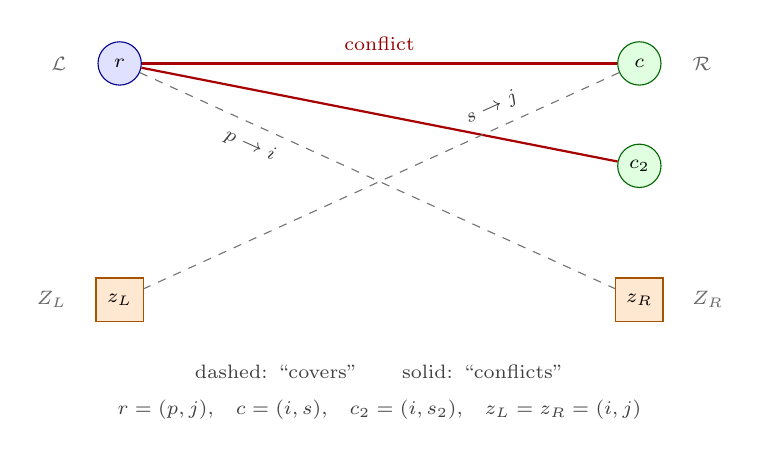
\begin{tikzpicture}[
  lv/.style={circle,draw=blue!55!black,fill=blue!12,minimum size=5.5mm,inner sep=0pt,font=\scriptsize},
  rv/.style={circle,draw=green!40!black,fill=green!12,minimum size=5.5mm,inner sep=0pt,font=\scriptsize},
  zv/.style={rectangle,draw=orange!65!black,fill=orange!18,minimum width=6mm,minimum height=5.5mm,inner sep=1pt,font=\scriptsize},
  conf/.style={draw=red!65!black,thick},
  cov/.style={draw=black!55,dashed},
  lab/.style={font=\scriptsize,text=black!75},
  grp/.style={font=\scriptsize\bfseries,text=black!60}
]
\node[lv] (r) at (0,3.2) {$r$};
\node[zv] (zl) at (0,0.2) {$z_L$};
\node[rv] (c) at (6.6,3.2) {$c$};
\node[rv] (c2) at (6.6,1.9) {$c_2$};
\node[zv] (zr) at (6.6,0.2) {$z_R$};
\node[grp,anchor=east] at (-0.55,3.2) {$\mathcal L$};
\node[grp,anchor=east] at (-0.55,0.2) {$Z_L$};
\node[grp,anchor=west] at (7.15,3.2) {$\mathcal R$};
\node[grp,anchor=west] at (7.15,0.2) {$Z_R$};
\draw[conf] (r) -- node[above=1pt,lab,text=red!60!black] {conflict} (c);
\draw[conf] (r) -- (c2);
\draw[cov] (c) -- node[near start,above=1pt,lab,sloped] {$s\to j$} (zl);
\draw[cov] (r) -- node[near start,below=1pt,lab,sloped] {$p\to i$} (zr);
\node[lab,anchor=north] at (3.3,-0.5) {dashed: ``covers''\qquad solid: ``conflicts''};
\node[lab,anchor=north] at (3.3,-0.95) {$r=(p,j)$,\quad $c=(i,s)$,\quad $c_2=(i,s_2)$,\quad $z_L=z_R=(i,j)$};
\end{tikzpicture}

\caption{The augmented bipartite graph $\Gamma$. \emph{Look at} the path
 $z_L-c-r-z_R$ forced by the conflict between $r=(p,j)\in\mathcal L$ and $c=(i,s)\in\mathcal R$,
 where $z=(i,j)$: the two dashed edges are the covering relations $s\to j$ and $p\to i$, the solid
 edges are conflicts. \emph{Why it matters:} conflicts and covering relations become edges of one
 bipartite graph, so that a single vertex cover pays for both: a conflict edge forces ``delete $r$ or
 delete $c$'', while a covering edge forces ``delete the member or spend the copy of $z$''. The
 second conflict drawn shares $r$, showing that the graph is not a disjoint union of such paths ---
 which is why a matching bound, not a path count, is needed.}
\label{fig:pruning-graph}
\end{figure}

\begin{lemma}[Matching bound]\label{lem:matching}
The maximum size $\nu(\Gamma)$ of a matching in $\Gamma$ satisfies
\[
 \nu(\Gamma)\le \abs Z+\abs H .
\]
\end{lemma}

\inwords{A maximum matching of the augmented graph has at most as many edges as there are conflict
points plus collisions.}

\begin{planbox}
\begin{enumerate}[leftmargin=1.3em,itemsep=1pt,topsep=1pt]
\item \textbf{Split the matching} (Step~2): choose a maximum matching $\mathcal M$ minimizing the
 number $k$ of original--original edges. Its other edges come in two families, $\alpha$ of size
 $\ell$ and $\beta$ of size $t$, and each of $\alpha,\beta$ is a maximum matching in its own
 subgraph.
\item \textbf{Encode by ranks} (Steps 3--5): build four matrices $L,N,A,B$ forming a commutative
 square $NL=AB$, and choose the coefficients so that $\rank L=\ell$, $\rank N^{\mathsf T}=t$ and
 some auxiliary matrices have maximum rank on their supports.
\item \textbf{Rank bookkeeping} (Step~4, used later): rank--nullity and the square give
 $\abs H\ge k+\ell+t-\abs Z$ as soon as $\dim\ker A\ge k$.
\item \textbf{Feed the kernel} (Steps 6--7): lift the $k$ original left endpoints to vectors
 $\lambda^r\in\ker L$ and show that their images $B\lambda^r$ are independent, using the rank lemma
 at the conflicting pairs.
\end{enumerate}
\end{planbox}

\begin{proof}
\steplabel{Step 1: the graph.}\label{step:gamma}
Throughout, $\Gamma$ is the augmented bipartite graph of \eqref{eq:Gamma}: its vertices are the
members of $\mathcal L$ and $\mathcal R$ together with the two copies $Z_L,Z_R$ of the conflict
points, and its edges are the conflicts and the covering relations. We must show that a matching of
$\Gamma$ has at most $\abs Z+\abs H$ edges.

\steplabel{Step 2: a maximum matching, split in three.}
Choose a maximum matching $\mathcal M$ of $\Gamma$ with as few edges as possible between two original
members. Write $k$ for the number of those edges, and let
\begin{equation}\label{eq:alpha-beta}
 \alpha=\mathcal M\cap(\mathcal L\times Z_R),\qquad
 \beta=\mathcal M\cap(Z_L\times\mathcal R),\qquad
 \ell=\abs\alpha,\qquad t=\abs\beta,
\end{equation}
so that $\abs{\mathcal M}=k+\ell+t$: these are the only kinds of edges of $\Gamma$.

\emph{$\alpha$ is a maximum matching between $\mathcal L$ and $Z_R$.} Suppose that subgraph had a
larger matching. Its symmetric difference with $\alpha$ contains an $\alpha$-augmenting path $P$
from an $\alpha$-unmatched member $r\in\mathcal L$ to an $\alpha$-unmatched vertex $z\in Z_R$. Every
internal vertex of $P$ is matched by $\alpha$, and $z$ is unmatched in $\mathcal M$ altogether
(because $z\in Z_R$ has neighbors only in $\mathcal L$, where $\mathcal M$ acts through $\alpha$).
If $r$ is unmatched in $\mathcal M$, augmenting along $P$ enlarges $\mathcal M$, which is impossible.
If $r$ is matched in $\mathcal M$, it is matched by an original--original edge (it is unmatched by
$\alpha$), and removing that edge and augmenting along $P$ keeps the size of $\mathcal M$ and lowers
$k$, contradicting the choice of $\mathcal M$. So no larger matching exists. The same argument with
the sides exchanged shows that $\beta$ is a maximum matching between $Z_L$ and $\mathcal R$. Write
$R_\alpha\subseteq\mathcal L$ and $C_\beta\subseteq\mathcal R$ for the original vertices matched by
$\alpha$ and by $\beta$.

\steplabel{Step 3: four matrices and the commutative square.}
For every arrow $x\to y$ of the relation introduce two \emph{independent} real variables
$a_{xy}$ and $b_{xy}$, and set an entry to $0$ whenever the corresponding arrow is absent. For any
assignment of the variables define four matrices
\begin{equation}\label{eq:fourmaps}
 \begin{array}{ccc}
 \R^{\mathcal L}&\xrightarrow{\ L\ }&\R^{Z}\\[2pt]
 {\scriptstyle B}\big\downarrow&&\big\downarrow{\scriptstyle N}\\[2pt]
 \R^{H}&\xrightarrow{\ A\ }&\R^{\mathcal R}
 \end{array}
 \qquad
 \begin{aligned}
  L_{(i,j),(p,j)}&=a_{pi},&\quad N_{(i,s),(i,j)}&=b_{sj},\\
  B_{(p,s),(p,j)}&=b_{sj},&\quad A_{(i,s),(p,s)}&=a_{pi},
 \end{aligned}
\end{equation}
all other entries being zero; the indices range over the indicated coordinate sets, so for instance
$L_{(i,j),(p,j)}$ is defined only for $(i,j)\in Z$ and $(p,j)\in\mathcal L$. The maps $L$ and $A$
advance the \emph{first} coordinate along an arrow $p\to i$; the maps $N$ and $B$ advance the
\emph{second} coordinate along an arrow $s\to j$. Two steps can be composed in two orders, and
\Cref{fig:fourmaps} shows that the two orders give the same result:
\begin{equation}\label{eq:commute}
 NL=AB .
\end{equation}
Indeed, the entry of $NL$ at $((i,s),(p,j))$ is $a_{pi}b_{sj}$ if $(i,j)\in Z$ and $0$ otherwise,
while the entry of $AB$ at the same place is $a_{pi}b_{sj}$ if $(p,s)\in H$ and $0$ otherwise. For
$(p,j)\in\mathcal L$ and $(i,s)\in\mathcal R$ the two conditions are equivalent: either both hold,
when the two members conflict, or neither does, and then $a_{pi}b_{sj}=0$ because at least one of
the two arrows is missing.

\begin{figure}[t]
\centering
\begin{tikzpicture}[
  sp/.style={font=\small},
  ar/.style={-{Stealth[length=2mm]},draw=black!70,thick},
  lab/.style={font=\scriptsize,text=black!75},
  note/.style={font=\scriptsize,text=black!60,align=center}
]
\node[sp] (L) at (0,2.4) {$\R^{\mathcal L}$};
\node[sp] (Z) at (6.0,2.4) {$\R^{Z}$};
\node[sp] (H) at (0,0) {$\R^{H}$};
\node[sp] (R) at (6.0,0) {$\R^{\mathcal R}$};
\draw[ar] (L) -- node[above=1pt,lab] {$L$} (Z);
\draw[ar] (L) -- node[left=1pt,lab] {$B$} (H);
\draw[ar] (H) -- node[below=1pt,lab] {$A$} (R);
\draw[ar] (Z) -- node[right=1pt,lab] {$N$} (R);
\node[lab,text=black!80,font=\normalsize] at (3.0,1.2) {$NL=AB$};
\node[note,anchor=east] at (-0.3,2.4) {indexed by\\ the left members};
\node[note,anchor=west] at (6.3,2.4) {indexed by\\ the conflict points};
\node[note,anchor=east] at (-0.3,0) {indexed by\\ the collisions};
\node[note,anchor=west] at (6.3,0) {indexed by\\ the right members};
\node[note,anchor=south] at (3.0,3.15) {$L$ and $A$ advance the first coordinate ($p\to i$)};
\node[note,anchor=north] at (3.0,-0.75) {$B$ and $N$ advance the second coordinate ($s\to j$)};
\end{tikzpicture}

\caption{The commutative square \eqref{eq:commute}. \emph{Look at} the two routes from
 $\R^{\mathcal L}$ to $\R^{\mathcal R}$: one goes through $\R^{Z}$, the other through $\R^{H}$, and
 the two composites agree. \emph{Why it matters:} this is the same square as the grid picture of
 \cref{fig:conflict} --- advancing the first coordinate and then the second, or the other way round,
 both take a left member to a right member, with intermediate cells $(i,j)\in Z$ and
 $(p,s)\in H$ --- and \eqref{eq:commute} is the only link between the matching $\mathcal M$ (whose
 pieces are counted by $Z$ and $H$) and the kernel of $A$ (which is where the $k$
 original--original edges are hidden).}
\label{fig:fourmaps}
\end{figure}

\steplabel{Step 4: rank bookkeeping.}
Suppose the coefficients are chosen so that
\begin{equation}\label{eq:rank-conditions}
 \rank L=\ell,\qquad \rank N^{\mathsf T}=t,\qquad \dim\ker A\ge k .
\end{equation}
Then, writing $\dim\ker A=\abs H-\rank A$ by rank--nullity,
\begin{align}
 \abs H&=\dim\ker A+\rank A\ge k+\rank A\ge k+\rank(NL)\notag\\
 &\ge k+\bigl(\ell-(\abs Z-t)\bigr)=k+\ell+t-\abs Z ,
 \label{eq:rank-bound}
\end{align}
where the second inequality uses $\im(NL)\subseteq\im A$ (from $NL=AB$) and the third restricts $N$
to $\im L$:
\begin{equation}\label{eq:rank-restrict}
 \rank(NL)=\dim\im L-\dim(\im L\cap\ker N)\ge\ell-(\abs Z-t),
\end{equation}
since $\dim\im L=\rank L=\ell$ and $\im L\cap\ker N\subseteq\ker N$ with
$\dim\ker N=\abs Z-\rank N=\abs Z-t$. Hence $\abs{\mathcal M}=k+\ell+t\le\abs Z+\abs H$, which is
the matching bound we need.

The first two conditions of \eqref{eq:rank-conditions} will come from $\alpha$ and $\beta$. The third
is the subtle one: it will be produced from the $k$ original--original edges, by finding $k$
independent vectors in $\ker A$.

\steplabel{Step 5: choosing the coefficients.}
We must justify that \eqref{eq:rank-conditions} can hold, together with one further family of rank
conditions, all at the same assignment. Two facts about ranks and matchings do all the work, and both
are proved in \appref{app:toolkit}:
\begin{itemize}[leftmargin=1.4em,itemsep=1pt,topsep=1pt]
\item \emph{a nonzero minor exhibits a matching} (\cref{lem:minor-matching}): a matrix supported on a
 set $T$ has rank at most $\nu(T)$, the largest number of entries of $T$ no two in a row or column;
\item \emph{an explicit matching gives an explicit maximal-rank matrix}: placing $1$s on the entries
 of a maximum matching and $0$s elsewhere produces a matrix of rank $\nu(T)$ supported on $T$,
 and every nonzero minor of such a matrix is a product of \emph{distinct} variables, hence a nonzero
 polynomial.
\end{itemize}
So for each of the matrices below we argue twice: an upper bound for \emph{every} assignment (no
support-matching is larger than the maximum matching we already have), and the existence of \emph{one}
assignment attaining it (an explicit minor whose determinant does not vanish identically). The
maximizing assignments of the various matrices must be combined, which is what (5d) does.

\emph{(5a) $\rank L=\ell$ with the columns $R_\alpha$ a basis of $\im L$.} For any assignment, a
nonzero $r\times r$ minor of $L$ needs $r$ entries no two in the same row or column and all nonzero,
i.e.\ a matching of size $r$ between $\mathcal L$ and $Z_R$; since $\alpha$ is maximum, $r\le\ell$ and
therefore $\rank L\le\ell$ always. For the reverse inequality consider the square minor with rows the
$Z$-endpoints of $\alpha$ and columns $R_\alpha$. Its entries $L_{(i,j),(p,j)}=a_{pi}$ vanish unless
the two second coordinates agree, so the minor is block diagonal with one block for each value of $j$.
Inside a block the only nonzero entries are the variables $a_{pi}$ of the matched pairs, one per row
and column, so the determinant is, up to sign, the product of those variables. Different permutations
of a block use different sets of variables, so no cancellation occurs: the determinant is a nonzero
polynomial in the $a$-variables. The determinant of the whole minor is the product of the block
determinants, up to sign (variables may occur in more than one block, but a product of nonzero
polynomials is nonzero). Hence at any assignment where this one polynomial does not vanish,
$\rank L=\ell$ and the columns $R_\alpha$ are independent, hence a basis of $\im L$.

\emph{(5b) $\rank N^{\mathsf T}=t$ with the columns $C_\beta$ a basis of $\im N^{\mathsf T}$.} The same
argument, with the roles of the two coordinates exchanged: the minor with rows the $Z$-endpoints of
$\beta$ and columns $C_\beta$ is block diagonal with one block per value of the \emph{first}
coordinate, each block determinant a product of distinct $b$-variables.

\emph{(5c) The auxiliary matrices.} For every arrow $p\to i$ of the relation put
\begin{equation}\label{eq:Dpi}
 J_p=\{j:(p,j)\in\mathcal L\},\qquad S_i=\{s:(i,s)\in\mathcal R\},
 \qquad D^{p,i}=(b_{sj})_{s\in S_i,\ j\in J_p} .
\end{equation}
So $D^{p,i}$ has rows indexed by $S_i$ and columns by $J_p$, and it is supported on
\begin{equation}\label{eq:Tpi}
 T^{p,i}=\{(s,j)\in S_i\times J_p:\ s\to j\}.
\end{equation}
For each arrow $p\to i$, choose a minor of $D^{p,i}$ that attains the maximum rank among matrices
supported on $T^{p,i}$; the entries of the minor are $b$-variables, so its determinant is a nonzero
polynomial in the $b$-variables, or the empty minor $1$ if that maximum rank is $0$. These matrices
are what connects the two kernels in Step~7: a conflict is exactly a triple with $(s,j)\in T^{p,i}$.

\emph{(5d) One assignment for everything.} Multiply the finitely many nonzero polynomials obtained in
(5a)--(5c). The product is a nonzero polynomial in the finitely many variables $a_{xy},b_{xy}$, since
the polynomial ring is an integral domain. A nonzero real polynomial in finitely many variables is
nonzero at some real point: induct on the number of variables, writing the polynomial as a polynomial
in the last variable whose coefficients are polynomials in the others. Fix once and for all a real
assignment at which the product does not vanish. At that assignment all the required minors are
nonzero simultaneously: $\rank L=\ell$ with $R_\alpha$ a basis of $\im L$, $\rank N^{\mathsf T}=t$
with $C_\beta$ a basis of $\im N^{\mathsf T}$, and every $D^{p,i}$ has maximum rank on $T^{p,i}$.

\steplabel{Step 6: lifting the original--original edges.}
For each original--original edge $(r,c)\in\mathcal M$, say $r=(p,j)\in\mathcal L$ and
$c=(i,s)\in\mathcal R$, the basis property of $R_\alpha$ provides coefficients $\xi^r_a$ with
\begin{equation}\label{eq:lifts}
 \lambda^r=e_r+\sum_{a\in R_\alpha}\xi^r_a\,e_a\in\ker L,
 \qquad
 \kappa^c=e_c+\sum_{b\in C_\beta}\eta^c_b\,e_b\in\ker N^{\mathsf T}.
\end{equation}
Such vectors exist because the column $Le_r$ of $L$ lies in $\im L=\Span\{Le_a:a\in R_\alpha\}$, so a
suitable linear combination of the $e_a$ cancels it. The endpoints $r$ and $c$ of an
original--original edge are matched by $\mathcal M$, hence not matched by $\alpha$ or $\beta$, so
$r\notin R_\alpha$ and $c\notin C_\beta$; consequently
\[
 \lambda^r_r=1,\qquad \lambda^r_{r'}=0\ \text{for every other original left endpoint }r',
 \qquad \kappa^c_c=1 .
\]

\steplabel{Step 7: the key vanishing, and $\dim\ker A\ge k$.}
The assertion to prove is
\begin{equation}\label{eq:key}
 u_{pj}\,v_{is}=0
 \qquad\text{for every conflict }\bigl((p,j),(i,s)\bigr),\quad
 u\in\ker B,\quad v\in\ker N^{\mathsf T}.
\end{equation}
Here $u\in\ker B\subseteq\R^{\mathcal L}$ and $v\in\ker N^{\mathsf T}\subseteq\R^{\mathcal R}$, so
the two factors are coordinates of the two vectors at the two conflicting members.

Fix an arrow $p\to i$ and $u\in\ker B$. The coordinate of $Bu=0$ at $(p,s)\in H$ reads
\begin{equation}\label{eq:row-eq}
 \sum_{j\in J_p}b_{sj}u_{pj}=0 .
\end{equation}
If a row $s\in S_i$ of $D^{p,i}$ has an allowed entry, choose $j\in J_p$ with $s\to j$; then $(p,j)$
and $(i,s)$ conflict (as $p\to i$), so $(p,s)\in H$ and \eqref{eq:row-eq} is exactly the statement
that the row $s$ of $D^{p,i}$ annihilates the vector $(u_{pj})_{j\in J_p}$. If the row has no allowed
entry, all its entries are $0$ and the same equation holds trivially. So
$(u_{pj})_{j\in J_p}\in\ker D^{p,i}$.

Similarly, for $v\in\ker N^{\mathsf T}$, the coordinate of $N^{\mathsf T}v=0$ at $(i,j)$ reads
\begin{equation}\label{eq:col-eq}
 \sum_{s\in S_i}b_{sj}v_{is}=0 ,
\end{equation}
which is the statement that $(v_{is})_{s\in S_i}$ is annihilated by the columns of $D^{p,i}$; the
coordinate $(i,j)$ is available in $Z$ whenever some $s\in S_i$ has $s\to j$, and the equation holds
trivially otherwise. So $(v_{is})_{s\in S_i}\in\ker(D^{p,i})^{\mathsf T}$.

Since $D^{p,i}$ has maximum rank on its support $T^{p,i}$, \cref{lem:kernel} applies to the two kernel
vectors and gives $u_{pj}v_{is}=0$ for every $(s,j)\in T^{p,i}$, i.e.\ whenever $s\to j$, which is
exactly \eqref{eq:key}. Note that the single-entry perturbation inside \cref{lem:kernel} is applied to
$D^{p,i}$ alone and need not preserve any other rank condition; the conclusion holds for the fixed
assignment of Step~5.

Now substitute $v=\kappa^c$ in \eqref{eq:key} for an original--original edge $(r,c)$ with $r=(p,j)$ and
$c=(i,s)$. Since $\kappa^c_c=1$, \eqref{eq:key} says $u_{pj}=0$ for every $u\in\ker B$: every vector of
$\ker B$ vanishes at $r$. Therefore the vectors $B\lambda^r$, for $r$ ranging over the $k$ original
left endpoints, are linearly independent. Indeed a relation $\sum_r\theta_rB\lambda^r=0$ puts
$u=\sum_r\theta_r\lambda^r$ in $\ker B$, and the coordinate of $u$ at each $r$ is $u_r=\theta_r$ by
\eqref{eq:lifts}; all these coordinates vanish, so all $\theta_r$ vanish. Moreover
\[
 A(B\lambda^r)=NL\lambda^r=0
\]
by \eqref{eq:commute}, because $\lambda^r\in\ker L$. So the $B\lambda^r$ are $k$ independent vectors
of $\ker A$, i.e.\ $\dim\ker A\ge k$. This is the third condition of \eqref{eq:rank-conditions}, and
Step~4 now gives $\abs{\mathcal M}\le\abs Z+\abs H$.

\end{proof}

\subsection{From the matching bound to the pruning}\label{sec:matching-to-pruning}

\begin{proof}[Proof of \cref{lem:pruning}]
If there is no conflict at all, keep every member; then $Z=H=\varnothing$ and
\eqref{eq:pruning-bound} is trivial. Otherwise build $\Gamma$ as in \eqref{eq:Gamma}.

\emph{An initially conflict-free member is isolated in $\Gamma$.} Let $(p,j)\in\mathcal L$ be
conflict-free and suppose it covers $(i,j)\in Z$. By definition of $Z$ there is a conflict between
some $(\tilde p,j)\in\mathcal L$ and some $(i,s)\in\mathcal R$; in particular $s\to j$. Then
$(p,j)$ and $(i,s)$ satisfy $p\to i$ and $s\to j$, so they conflict, contrary to the assumption.
The same argument with the sides exchanged applies to $\mathcal R$. So conflict-free members have
no edges at all.

\emph{A cover gives the bound.} By \cref{thm:konig} (proved in \appref{app:toolkit}) the graph
$\Gamma$ has a vertex cover $K$ with $\abs K=\nu(\Gamma)\le\abs Z+\abs H$ that contains exactly one
endpoint of each edge of a maximum matching and no unmatched vertices; in particular it contains no
isolated vertex. Delete exactly the original members lying in $K$. Since $K$ covers every edge, no
conflict survives, and since $K$ contains no isolated vertex, no initially conflict-free member is
deleted. Let $q$ be the number of points of $Z$ covered by no surviving member. Each of the other
$\abs Z-q$ points $z\in Z$ is covered by some surviving member; that member is adjacent to one of
the two copies of $z$, so that copy lies in $K$, because the edge between them is not covered from
the other side (the member is not in $K$). Distinct points have distinct copies, so
\begin{equation}\label{eq:cover-charge}
 \abs{K\cap(\mathcal L\sqcup\mathcal R)}
 \le\abs K-(\abs Z-q)\le\abs H+q ,
\end{equation}
which is \eqref{eq:pruning-bound}. \Cref{fig:cover} records the counting.
\end{proof}

\begin{figure}[t]
\centering
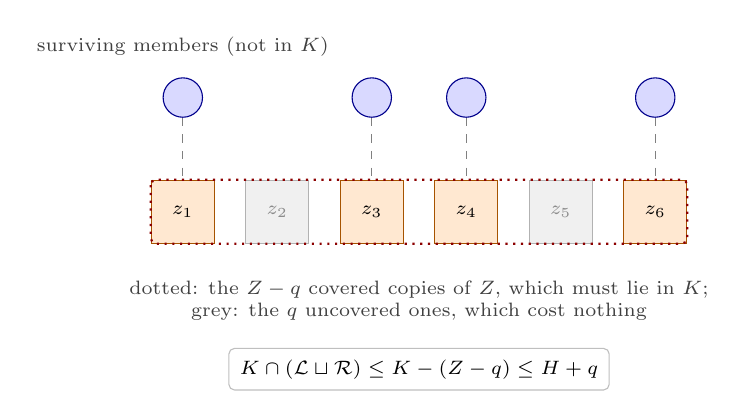
\begin{tikzpicture}[
  zv/.style={rectangle,draw=orange!65!black,fill=orange!18,minimum width=8mm,minimum height=8mm,inner sep=0pt,font=\scriptsize},
  unc/.style={rectangle,draw=black!30,fill=black!6,minimum width=8mm,minimum height=8mm,inner sep=0pt,
              font=\scriptsize,text=black!45},
  mem/.style={circle,draw=blue!55!black,fill=blue!15,minimum size=5mm,inner sep=0pt},
  cov/.style={draw=black!50,dashed},
  lab/.style={font=\scriptsize,text=black!75}
]
\node[zv]  (z1) at (0.0,0) {$z_1$};
\node[unc] (z2) at (1.2,0) {$z_2$};
\node[zv]  (z3) at (2.4,0) {$z_3$};
\node[zv]  (z4) at (3.6,0) {$z_4$};
\node[unc] (z5) at (4.8,0) {$z_5$};
\node[zv]  (z6) at (6.0,0) {$z_6$};
\node[mem] (m1) at (0.0,1.45) {};
\node[mem] (m3) at (2.4,1.45) {};
\node[mem] (m4) at (3.6,1.45) {};
\node[mem] (m6) at (6.0,1.45) {};
\foreach \a/\b in {m1/z1,m3/z3,m4/z4,m6/z6}{ \draw[cov] (\a) -- (\b); }
\draw[red!55!black,dotted,thick,rounded corners=2pt] (z1.north west) rectangle (z6.south east);
\node[lab,anchor=south] at (0.0,1.85) {surviving members (not in $K$)};
\node[lab,anchor=north,align=center] at (3.0,-0.75)
  {dotted: the $\abs Z-q$ covered copies of $Z$, which must lie in $K$;\\
   grey: the $q$ uncovered ones, which cost nothing};
\node[draw=black!25,fill=white,rounded corners=2pt,inner sep=4pt,font=\scriptsize]
  at (3.0,-2.0) {$\abs{K\cap(\mathcal L\sqcup\mathcal R)}\le\abs K-(\abs Z-q)\le\abs H+q$};
\end{tikzpicture}

\caption{The counting behind \eqref{eq:cover-charge}. \emph{Look at} the row of copies of the points
 of $Z$: the $q$ points left uncovered cost nothing, and each of the remaining $\abs Z-q$ must have a
 copy in $K$ because the edge from it to its surviving member is not covered from the other side.
 \emph{Why it matters:} this is the only place where the ``uncovered'' term of the pruning bound comes
 from, and it is why the bound degrades gracefully: the more the survivors leave uncovered, the less
 the cover has to pay for the points of $Z$.}
\label{fig:cover}
\end{figure}

\begin{checkpoint}
The lemma is proved. Three sentences to keep: \emph{conflicts and covering relations become edges of
a bipartite graph $\Gamma$}; \emph{K\"onig turns a bound on the maximum matching of $\Gamma$ into a
vertex cover of the same size, and deleting its original members is the pruning}; \emph{a maximum
matching has at most $\abs Z+\abs H$ edges, because the two coverage matchings $\alpha,\beta$ and the
$k$ original--original edges are three quantities that ranks can count, and the commuting square
$NL=AB$ forces the $k$ lifts into the kernel of $A$}. The next section applies the lemma to the
families produced by the subset inequalities of \cref{sec:reduction}.
\end{checkpoint}

\begin{remark}[What the rank argument is really doing]\label{rem:rank-philosophy}
It is worth separating the three roles of linear algebra in Steps 3--7, because the proof is easy to
read as a sequence of tricks.
\begin{enumerate}[leftmargin=1.3em,itemsep=2pt,topsep=1pt]
\item \textbf{Rank as a matching counter.} The maximum rank of a matrix supported on a set $T$ equals
  the maximum size of a matching in $T$; only the easy direction is needed
  (\cref{lem:minor-matching}): a nonzero
  minor exhibits a matching, so $\rank\le$ matching size; and the explicit minors of (5a), (5b) are
  chosen to \emph{achieve} the matching bound. Thus $\rank L=\ell$ is a certificate that
  $\alpha$ is maximum, and $\rank N^{\mathsf T}=t$ that $\beta$ is.
\item \textbf{Rank--nullity as a trade-off.} If a matrix from a space of dimension $\abs H$ has rank
  $r$, its kernel has dimension $\abs H-r$. So a lower bound on the kernel is an upper bound on the
  rank, hence on a matching. This is the chain \eqref{eq:rank-bound}: $\dim\ker A\ge k$ and
  $\rank A\ge\rank(NL)$ together give $\abs H\ge k+\ell+t-\abs Z$.
\item \textbf{The commuting square as incompatibility.} The identity $NL=AB$ says that a conflict can
  be traversed in two ways. If both a left kernel vector and a right kernel vector were nonzero at the
  two ends of a conflict, the two routes would force a contradiction, and the rank lemma turns that
  into the vanishing \eqref{eq:key}. That vanishing is what makes $k$ vectors out of nothing: the
  right kernel vector $\kappa^c$ kills the coordinate of every left kernel vector at $r$.
\end{enumerate}
\end{remark}
